\documentclass[11pt,letterpaper]{article}

\usepackage[letterpaper,margin=0.75in,nohead]{geometry}
\usepackage{verbatim}
\usepackage[colorlinks]{hyperref}
\usepackage{url}
\usepackage{hyperref}
\usepackage{breakurl}
\usepackage[T1]{fontenc}
\usepackage{graphicx} %package to manage images
\usepackage{placeins} %For floatbarrier
\graphicspath{ {./tables/}}
\usepackage{caption}
\usepackage{subcaption}

% \usepackage[document]{ragged2e}

\hypersetup{
    colorlinks,
    linkcolor={blue},
    citecolor={red},
    urlcolor={blue}
}

% \addtolength{\topmargin}{-0.1in}

% add packages as needed
% testing

\title{CIS 6930: Trustworthy Machine Learning\\
	\Large Final Report: Machine Unlearning for Randomized Decision Trees} %% TODO: replace with the title of your project

%% TODO: your name and email go here (all members of the group)
%% Comment out as needed and designate a point of contact
\author{
        Ashwin Rai \\{\em (Point of Contact)} \\ 
        raiashwin@ufl.edu\\
        \and
        Vaibhav Kulkarni \\
        kulkarniv@ufl.edu\\
        \and
        Zubin Arya \\
        z.arya@ufl.edu\\
}

% set the date to today
\date{\today}


\begin{document} % start document tag

\maketitle


\begin{abstract}

Computational feasibility is an important aspect while updating the model for retraining when user requests digital footprint from the dataset to be removed. It is obvious that it is not feasible to retrain the model from scratch for large datasets if every time selected data points are purged. To make model update computationally feasible, machine unlearning comes to the rescue. Since there has been limited scope of work done for machine unlearning on tree based models, we came up with study of machine unlearning on data removal-enabled forest (DaRE) models which is a variant of the random forest and focused on three quantifying metrics to evaluate the efficacy of the machine unlearning with respect to complete retraining which are data deletion threshold, space overhead and the time overhead.

% focus on data deletion taking into account three datasets out of which one dataset app behaviour was taken as a validate dataset which was not done in the bropy research paper.

\end{abstract}

\vspace{-5mm} %Just pretend this isn't here we couldn't fit the table of contents on one page smh 

%Also, Franny had to google smh to learn what it means

%When you are editing this project to start writing your paper, just delete or comment out the table of contents, or keep it if you like seeing an outline generated of what you are writing. To see what a ``comment'' is, read the introduction below!

\tableofcontents

\clearpage

%%% Remember: writing counts! (try to be clear and concise.)
%%% the whole proposal should be about 2 pages (in 11pt font)


%% TODO: write your introduction

%% Must address:
%% - What is the problem?
%% - Why is the problem interested and worth solving?
%% - What are you proposing to do (at high level)?
%%
\section{Introduction}

% TODO:

% right to be forgotten -

% Removed the below point in the second part of the introduction
There is a rising need for users to safeguard their footprints by forcing search engines to remove their links about them from the past. The  \emph{Right to be forgotten} law which is General Data Protection Regulation(GDPR) and  California Consumer Privacy Act(CCPA) addresses these issues and strives to enforce security and maintain the privacy of both individuals and community by and large.
\smallskip

Large organizations that consume and process public data are obligated to respect these laws and maintain the privacy and security of the users. In most cases, the organizations train machine learning models on these large data sets, and the problem arises when a part of the training data set decides to move out of the system and requests to erase their data, data lineage, any traces of their data along with its influence or contribution in training the machine learning model. Organizations around the world use diverse strategies to implement machine unlearning. A naive approach is to retrain a model from scratch, but it becomes computationally and resourcefully expensive in the case of large datasets.
\smallskip

% This project plans to take up a specific machine learning model type and implement techniques specifically for randomized decision tree models without retraining the whole model. We will also test multiple case scenarios on different data sets and validate results for unlearning.

In this project, we have chosen variant of randomized decision tree machine learning model which is DaRE and implemented machine unlearning without retraining the whole model. In the subsequent sections, we will evaluate computational feasibility and robustness of the machine unlearning using DaRE model against complete retraining. For evaluation, we will use quantifying metrics which are unlearning time computation, space overhead and effect of tuning hyper-parameters. In addition, we will test the membership inference attacks on the deleted instances to validate the claim of guaranteed unsuccessful membership inference attacks on deleted instances.

% ---------------------////////-----------------------

\section{Background and Related Work}
During the process of the work survey, we studied numerous pieces of literature, and we observed multiple approaches and strategies being used to achieve machine unlearning. For this project, we decided to work on the specific machine learning model type, the randomized decision tree. We referred to the paper ``Humans Forget, Machines Remember" \cite{eduardf1} to clearly understand and learn the legal background behind the Right to Be Forgotten. The technical papers that are strongly related to unlearning of Randomised decision tree were ``Brophy and Lowd, Machine Unlearning for Random Forests" \cite{Brophy} and ``Schelter et al. HedgeCut: Maintaining Randomised Trees for Low-Latency Machine Unlearning" \cite{Schelter} which emphasize on ensembling of small randomized decision trees to achieve low latency machine unlearning for classification type problems. We also referred to the literature ``DART: Data Addition and Removal Trees" \cite{BrophyDart} which proposes a variant of Random Forests that supports the addition or removal of data. We believe ``HedgeCut" and ``data removal-enabled forests" (DaRE) are some of the efficient unlearning techniques developed for tree-based models. 

Based on our findings from the above cited research papers especially, we were motivated to investigate further into the machine unlearning for DaRE models implemented in this paper \cite{Brophy} with focus on three key aspects. First is the operating limits and robustness of the unlearning solution by finding the threshold up to which data points can be removed while retaining the accuracy of the model in comparison to the completely retrained model. Secondly, to test the feasibility of the batch deletion through successive single instance deletions and validate claims of membership inference attacks.

% First of all, we will test the operating limits and robustness of the unlearning solution by finding the threshold up to which data points can be removed while retaining the accuracy of the model in comparison to the completely retrained model. Secondly, we will also test the feasibility of the batch deletion through successive single instance deletions.

% TODO:

% You can cite related publications like so~\cite{vapnik1994measuring} and non-publications (e.g., websites) like so\footnote{Google scholar: \url{https://scholar.google.com}}.


%% TODO: write your proposed approach and describe your plan
%%
%% - Describe your approach to solve the problem
%% - What's your plan?
%% - Be concrete!!
%% 		-- What dataset will you use?
%% 		-- What equipment do you need? How will you get it?
%% 		-- What are you going to measure? What metrics will you use?
%%		-- How will you know whether what you are doing is working?
%% 
\section{Approach}
We analyzed and studied the frameworks DARE and DART, thereby refactoring the strategy to build a model with support for single instance deletion unlearning and batch unlearning through sequential deletion.

For the computation and building of the model, we have used the local system running on Ubuntu 20.2 with Intel i5-10600K processor,16 GB memory and NVIDIA 3070ti Graphics.

We measure the speedup of the generated unlearned model in comparison with the completely retrained model. Speedup is the ratio of time for generating the model (unlearning vs. retraining). We evaluate the delta between the unlearned model and retrained model accuracy on the test data. We choose random data points to be deleted uniformly. We aim to achieve speedup by a factor of two on average and have delta error within 5\% with respect to the unlearned vs. retrained model.

\subsection{Dataset(s)}
We plan to work with the following privacy-sensitive datasets:
\href{https://archive.ics.uci.edu/ml/datasets/adult}{Census Income Dataset}\footnote{Census Income Dataset Link: \url{https://archive.ics.uci.edu/ml/datasets/adult}} which predicts whether the annual income of an individual exceeds 50k USD, based on census data. \href{https://archive.ics.uci.edu/ml/datasets/bank+marketing}{Bank Marketing Dataset}\footnote{Bank Marketing Dataset Link: \url{https://archive.ics.uci.edu/ml/datasets/bank+marketing}} which predicts whether the client will subscribe a term deposit or not and \href{https://www.kaggle.com/hkhamnakhalid/customers-to-subscription-through-app-behavior}{App Behavior Dataset}\footnote{App Behavior Dataset Link: \url{www.kaggle.com/hkhamnakhalid/customers-to-subscription-through-app-behavior}} which predicts new customer who is interested in buying the product or not.

\subsection{Plan of Action}
\begin{itemize}
    \item We started with the technical analysis of the paper referenced Jonathan Brophy and Lowd Daniel on Machine unlearning for random forests \cite{Brophy}. We built our own version of DaRE and implemented in python and built its relevant dependencies.
    \item In addition to the datasets used in the experimentation,
    we chose our own new dataset. \href{https://www.kaggle.com/hkhamnakhalid/customers-to-subscription-through-app-behavior}{App Behavior Dataset} which was not used in the original experimentation, to validate the claims. 
    \item Through experimentation, we determined the optimal size of the dataset (threshold) which can be unlearned for which unlearning time is less than the retraining time, which was not originally covered in the scope of the paper by Jonathan Brophy and Lowd Daniel \cite{Brophy}.
    \item We performed time and space overhead analysis and tuned the hyperparameters ($d_{rmax}$ and $k$) to improve the speedup and potentially extended the threshold for optimal deletion size.
    \item  In addition, we validated the claim \textit{deletions in random forest are exact, so Membership Inference attack is guranteed to be unsuccessful} by implementing Membership Inference attack on DaRE model which was a part of discussion and left for future scope.
\end{itemize}


\subsection{Experiments and Validations}

\begin{itemize}
    \item After successfully implementing the DaRE, we performed the unlearning experiments for three data sizes, ie. \textbf{small}, \textbf{medium} and \textbf{large} for each dataset used for experimental purpose.
    \item Originally the DaRE model was overfitted on \textbf{app behavior analysis}, we tuned the parameters to avoid the overfitting.
    \item We faced some \textbf{challenges} in experimenting with the \textbf{app behaviour analysis} after data preprocessing using \textbf{columntransformer} with kmeansdiscretizer, we obtained large number of columns with one hot encoding which required high compute time for model training. We resolved this issue by performing data visualization followed by feature selection which successfully reduced the computation time.
    \item We tuned the following hyperparameters which are the maximum depth of each tree $d_{max}$ (greedy) and $d_{rmax}$ (random) , the number of trees in the forest T and the number of thresholds considered per attribute for greedy nodes $k$.
    \item From the previous work done by Brophy and Daniel and from our own experiments we identified that increasing $d_{rmax}$ (random) and reducing $k$, can improve the speedup of the DaRE at the cost of small loss in the predictive performance for small number of unlearning samples (>1\%) and for large data deletions, we keep tuning the hyper parameters to produce similar results and to obtain optimal values of  $d_{rmax}$ and $k$ respectively.
    \item Space Overhead Computation: To test the impact of space consumption, we performed the space overhead analysis by comparing our version of DaRE with the ScikitLearn random forest.
    \item Implementation of Membership Inference Attack: We performed two attacks which are Shokri attack and Loss attack 2. We took into account all three datasets and trained the samples. We deleted some samples used in the training set from the each of the datasets and evaluated above chosen Membership Inference attacks on the deleted samples to check whether they were able to predict whether these samples were a part of the training set or not.
    % \item We will put additional tabular results here -space overhead, hyperparameter tuning results DONE
    
\end{itemize}
\begin{figure}[h]
         \centering
             \centering
             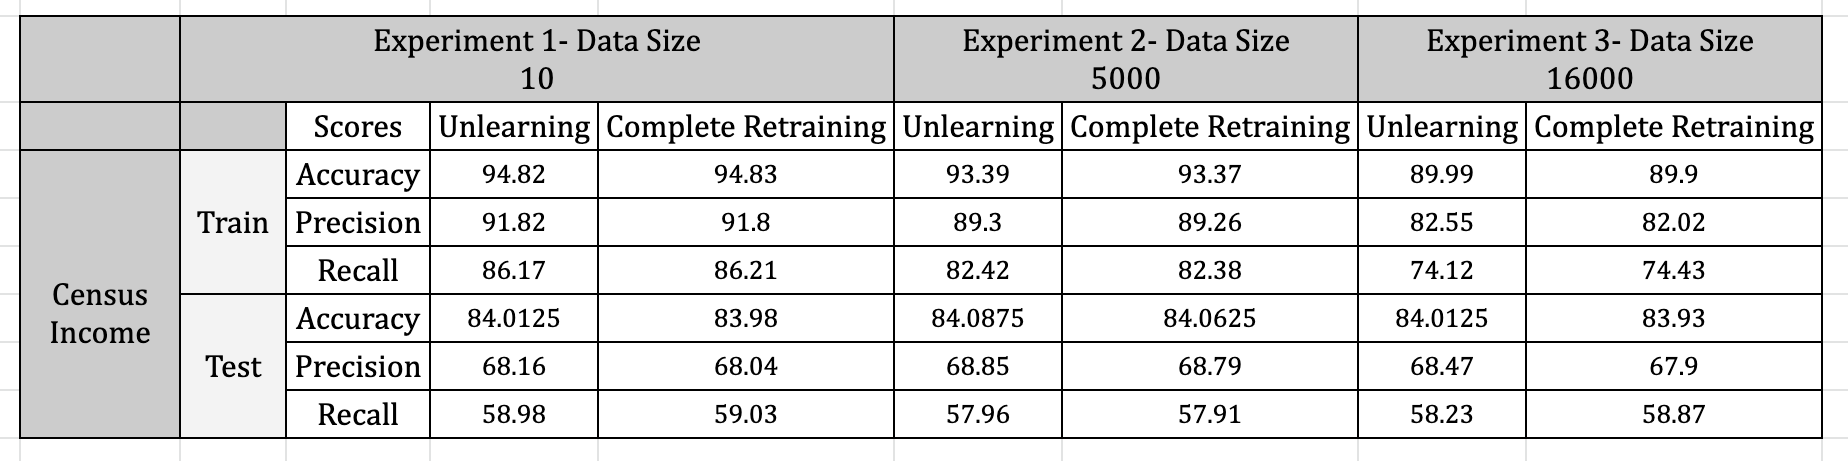
\includegraphics[width=\textwidth]{tables/Census-Income.png}
             \caption{Census Income Dataset: Unlearning vs Retraining results}
             \footnotesize
             \label{fig:censusincome-results-1}
\end{figure}

\begin{figure}[h]
         \centering
             \centering
             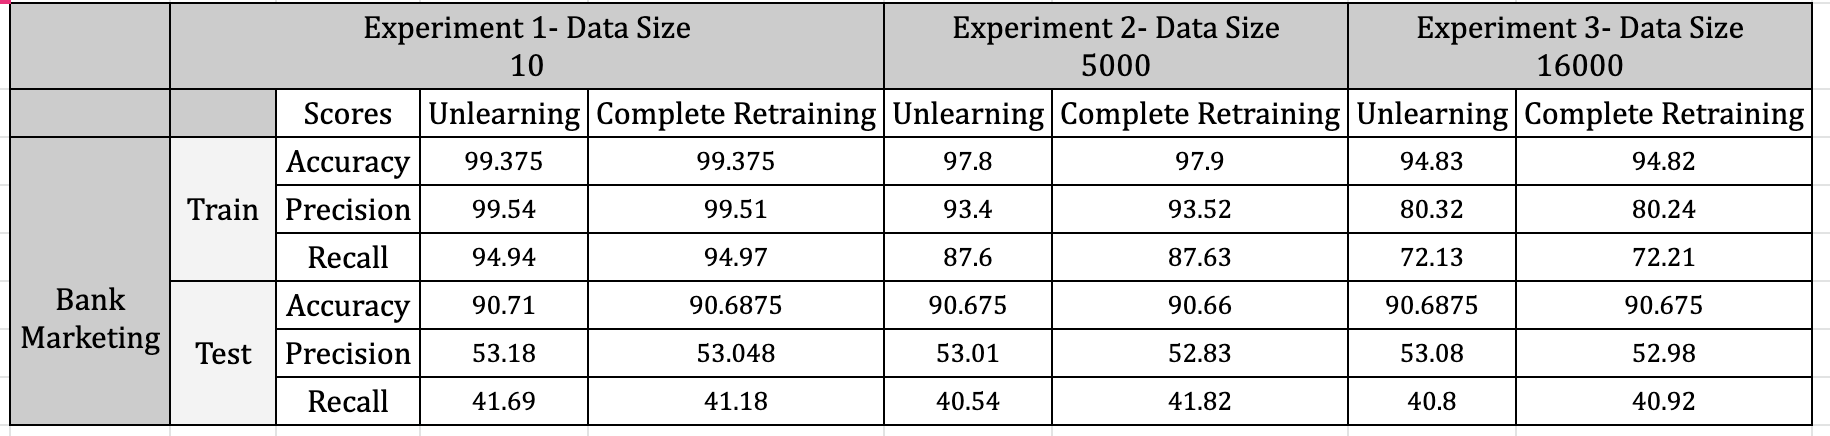
\includegraphics[width=\textwidth]{tables/Bank-Marketing.png}
             \caption{Bank Marketing Dataset: Unlearning vs Retraining results}
            %  \label{fig:bankmarketing-results-1}
             \footnotesize
             \label{fig:bankmarketing-results-1}
\end{figure}

\begin{figure}[h]
         \centering
             \centering
             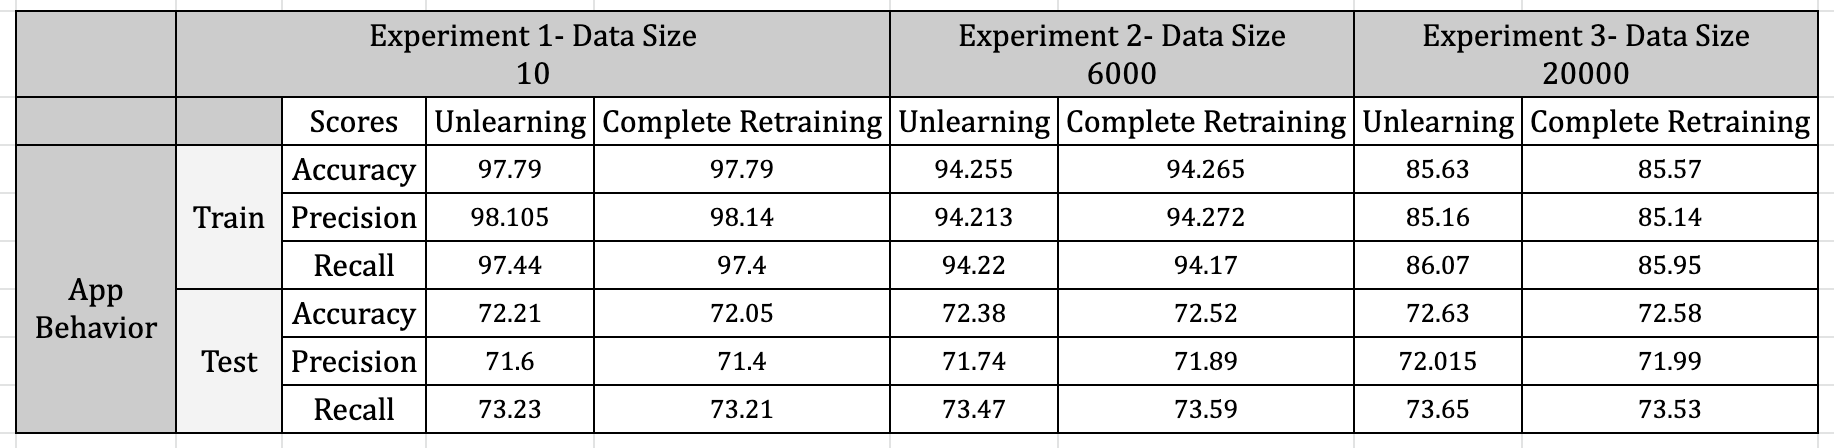
\includegraphics[width=\textwidth]{tables/App-Behaviour.png}
             \caption{App Behaviour Dataset: Unlearning vs Retraining results}
            %  \label{fig:appbehaviour-results-1}
             \footnotesize
             \label{fig:appbehaviour-results-1}
             %\caption{Experimental results in (\%)}
\end{figure}

\begin{figure}[h]
    \centering
    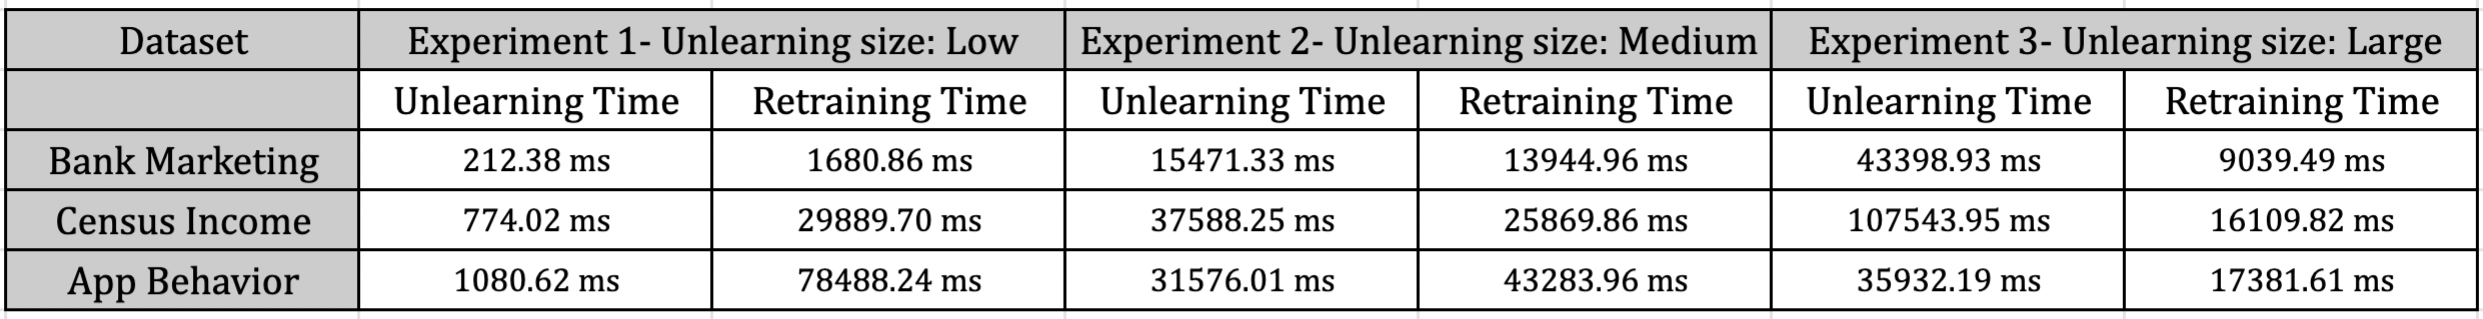
\includegraphics[width=\textwidth]{tables/SpeedupTime.png}
    \caption{Speedup Time for Unlearning vs Retraining in (ms)}
    \label{fig:speeduptime}
\end{figure}

\begin{figure}[h]
\centering
\begin{subfigure}{.5\textwidth}
  \centering
  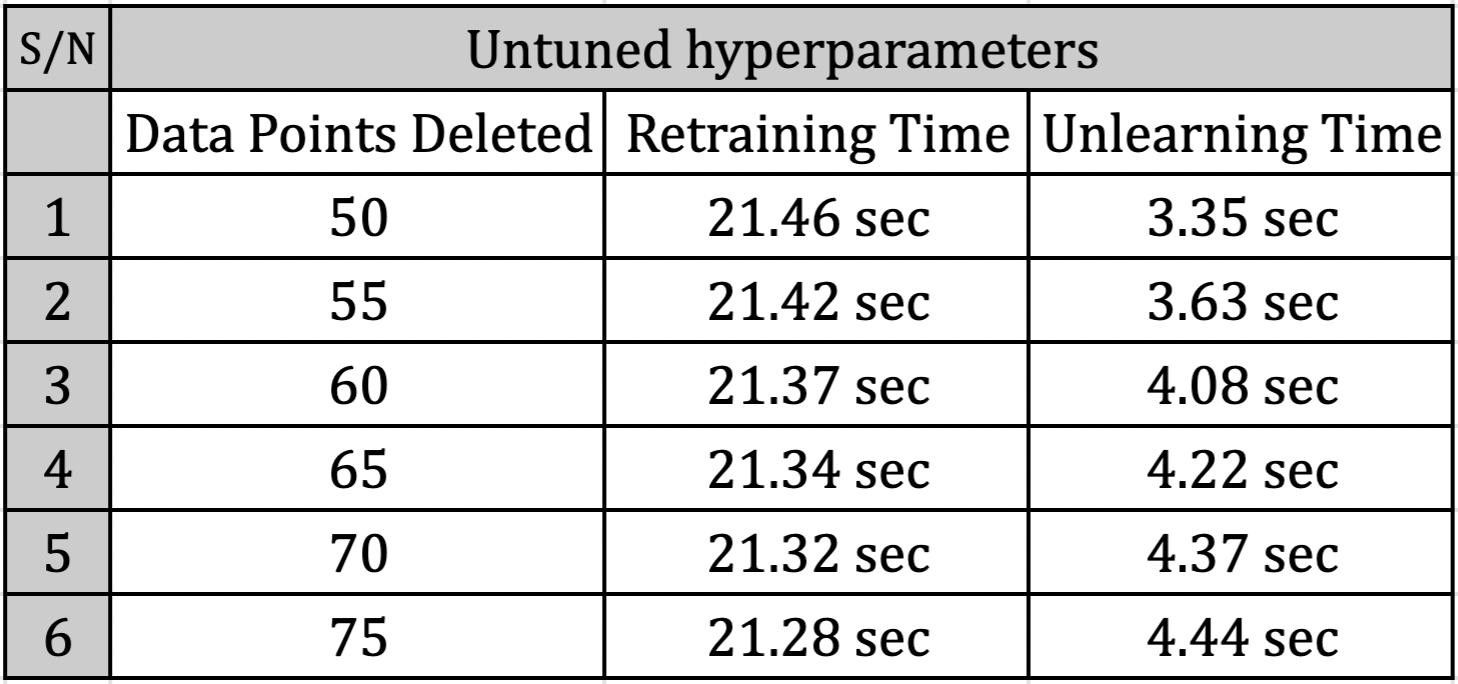
\includegraphics[width=.9\linewidth]{tables/Params_Untuned.png}
  \caption{Parameter Untuned}
  \label{fig:sub1}
\end{subfigure}%
\begin{subfigure}{.5\textwidth}
  \centering
  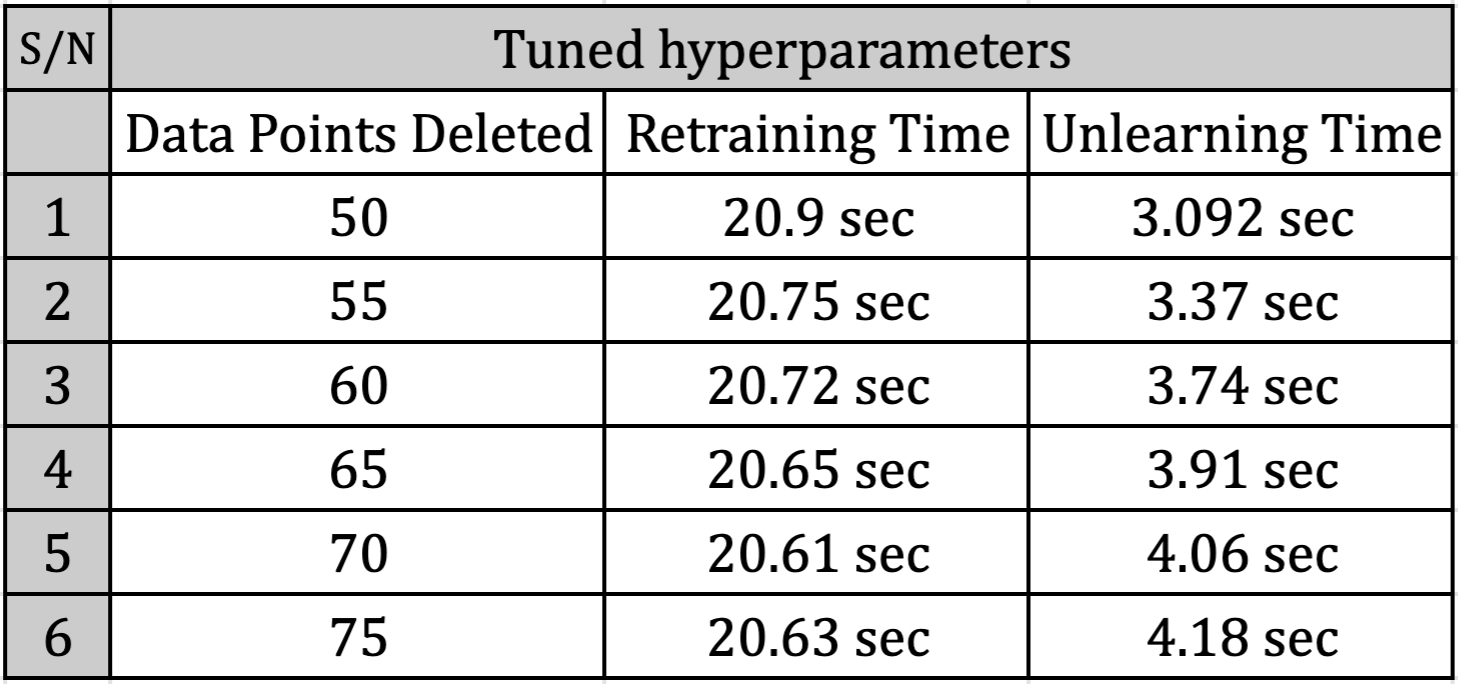
\includegraphics[width=.9\linewidth]{tables/Params_Tuned.png}
  \caption{Parameter Tuned}
  \label{fig:sub2}
\end{subfigure}
\caption{App Behaviour Dataset: Observed Speedup in unlearning post tuning parameters}
\label{fig:paramtuning}
\end{figure}

\begin{figure}[h]
    \centering
    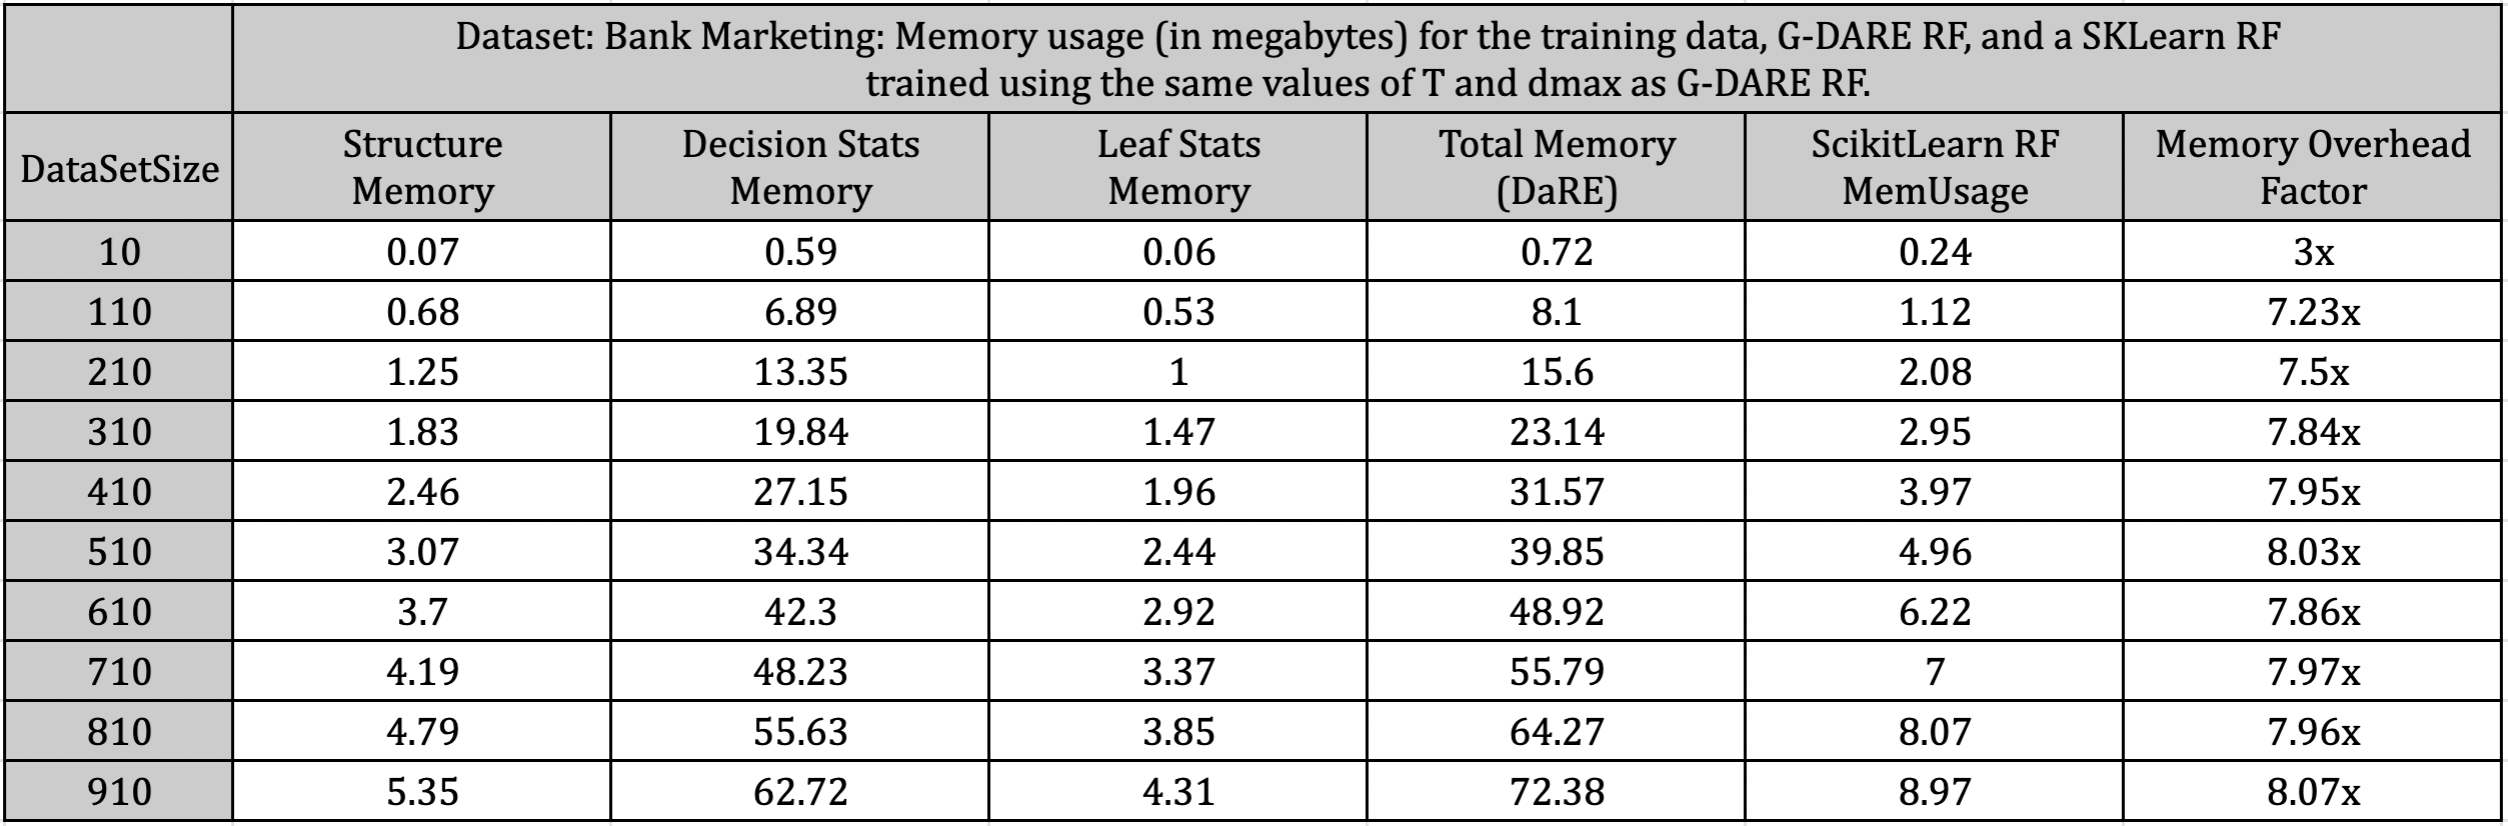
\includegraphics[width=\textwidth]{tables/Memory_Bank_Marketing.png}
    \caption{Bank Marketing Dataset: Memory usage (MB) comparison of Total Memory(DaRE) vs Standard Random Forest by ScikitLearn}
    \label{fig:memusagebankmarketing}
    \end{figure}

    \begin{figure}[h]
    \centering
    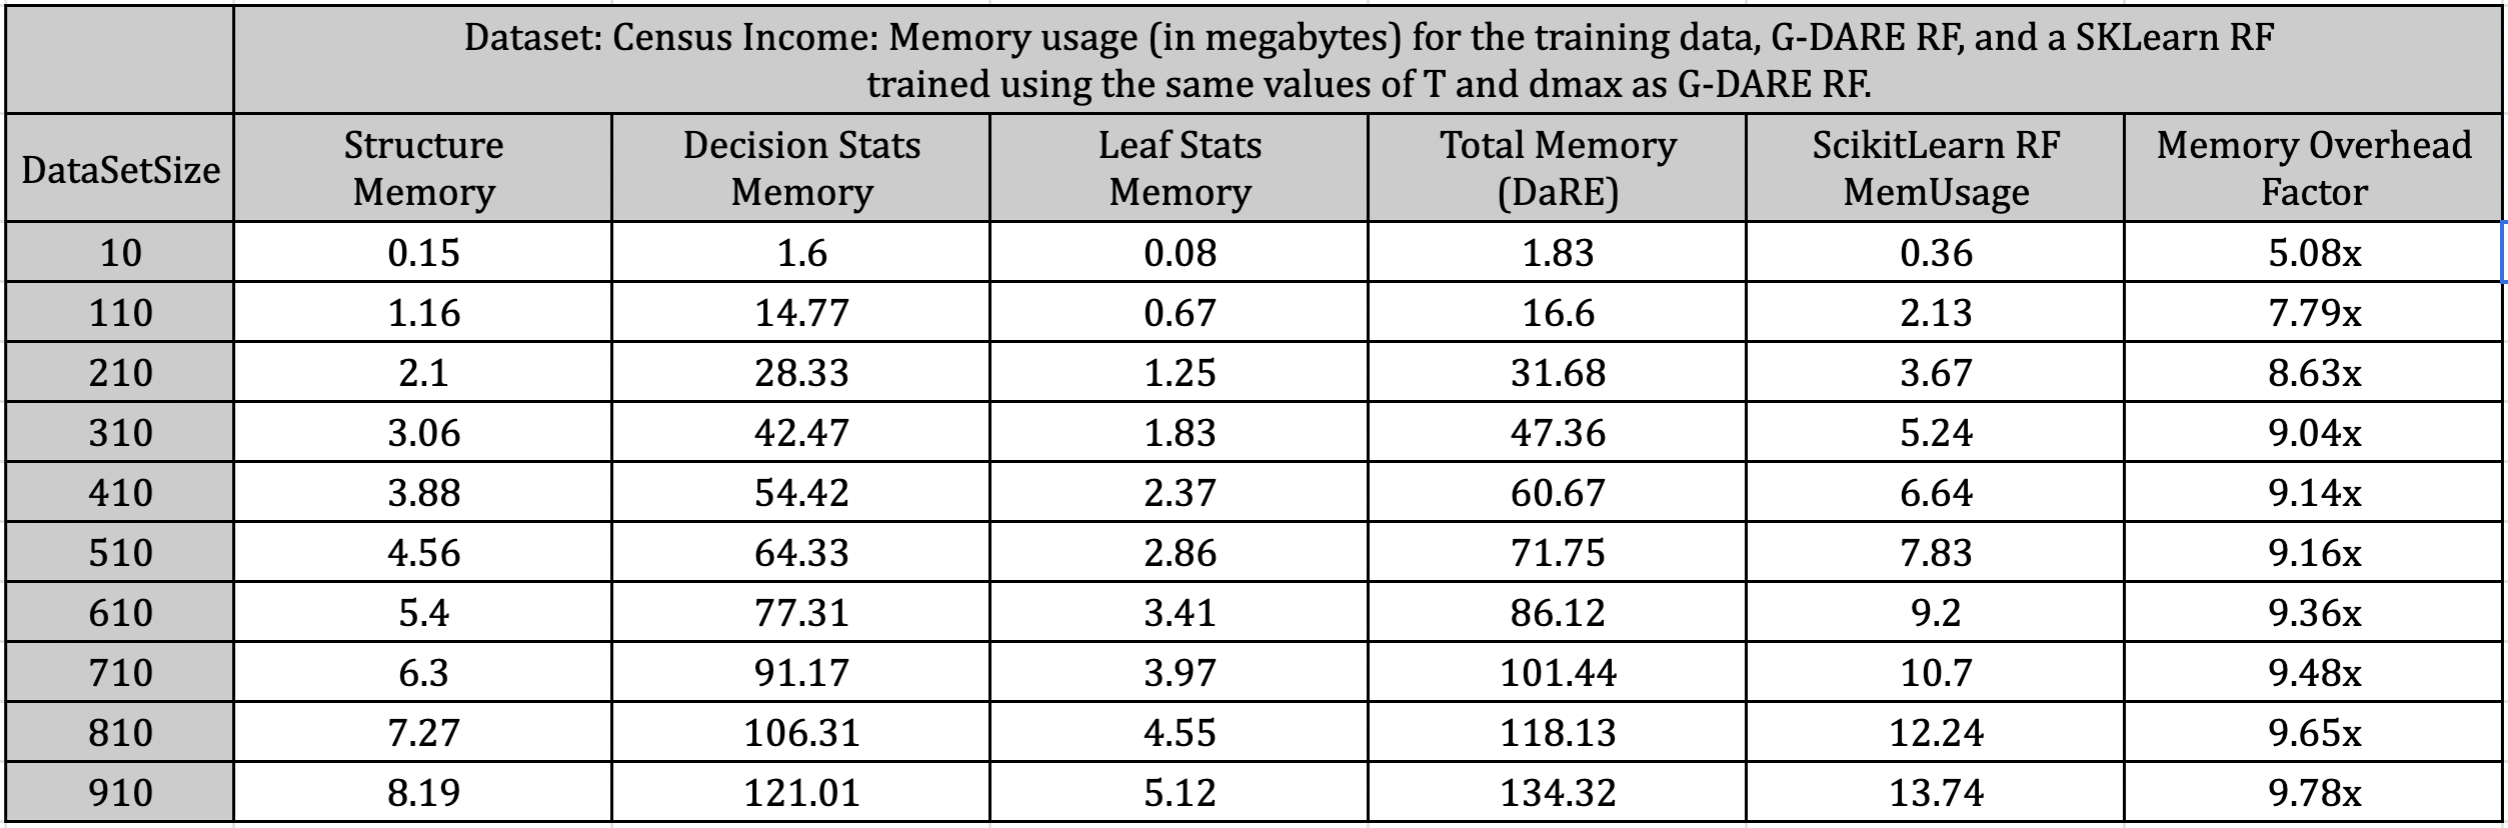
\includegraphics[width=\textwidth]{tables/Memory_Census.png}
    \caption{Census Income Dataset: Memory usage (MB) comparison of Total Memory(DaRE) vs Standard Random Forest by ScikitLearn}
    \label{fig:memusagecensusincome}
    \end{figure}

    \begin{figure}[h]
    \centering
    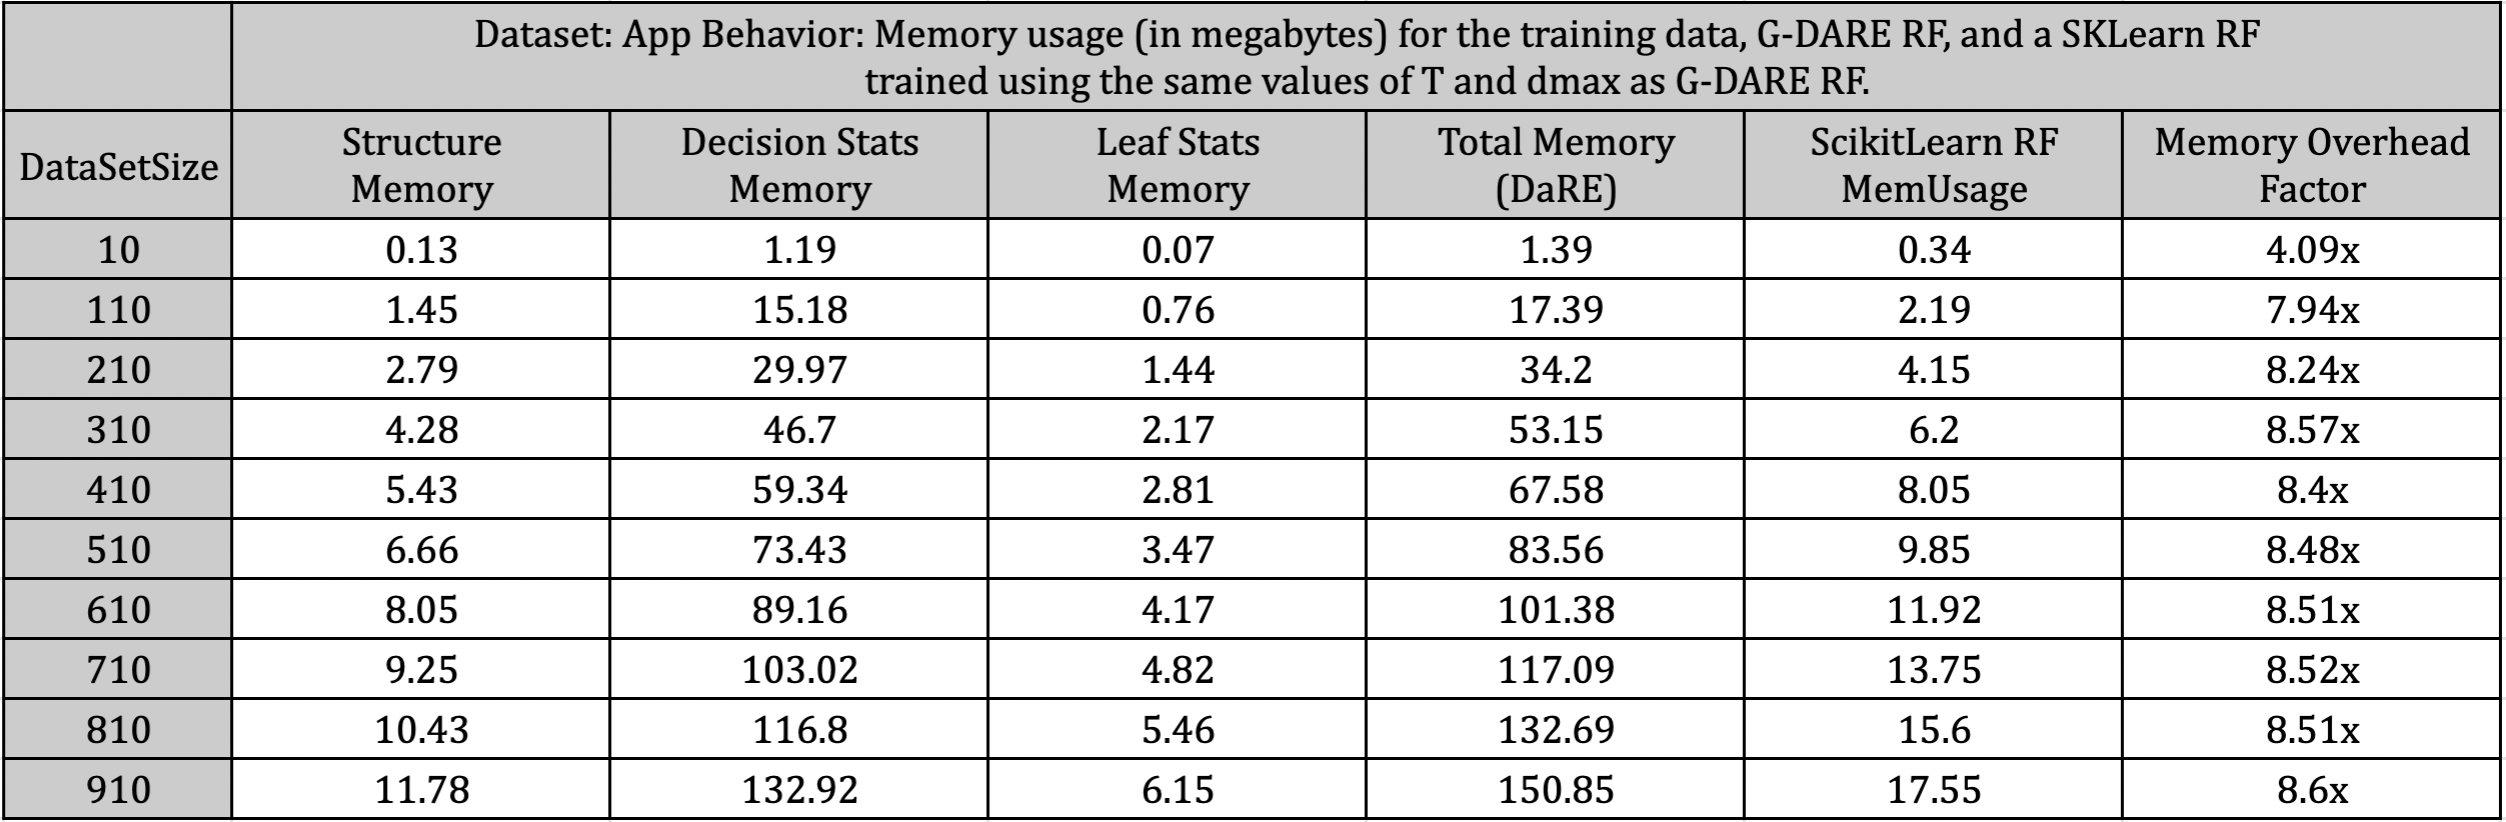
\includegraphics[width=\textwidth]{tables/Memory_App_Behavior.png}
    \caption{App Behaviour Dataset: Memory usage (MB) comparison of Total Memory(DaRE) vs Standard Random Forest by ScikitLearn}
    \label{fig:memusageappbehviour}
\end{figure}
    
% \FloatBarrier

\begin{figure}[h]
    \centering
    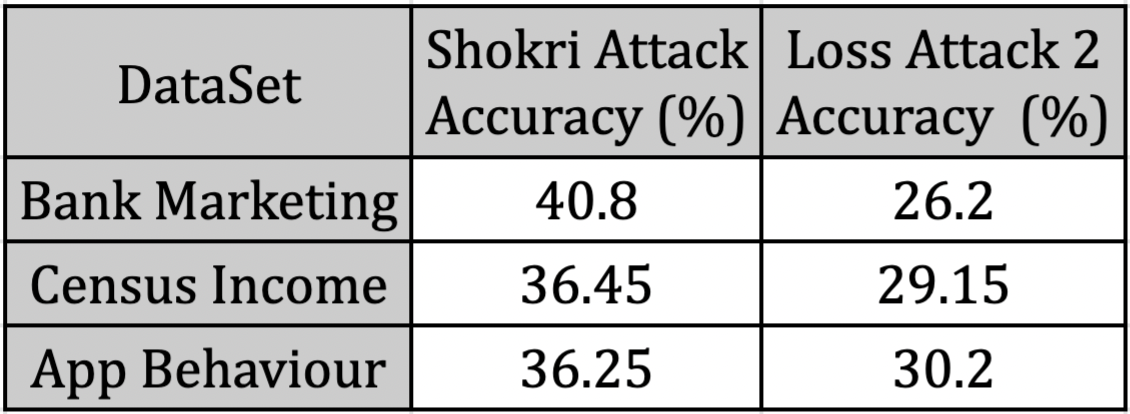
\includegraphics[width=3 in]{tables/MIA_Results.png}
    \caption{Membership Inference Attack: Accuracy Comparison of Shokri and Threshold Loss Attack on three datasets}
    \label{fig:MIA-attacks}
\end{figure}

\begin{figure}[h]
    \centering
    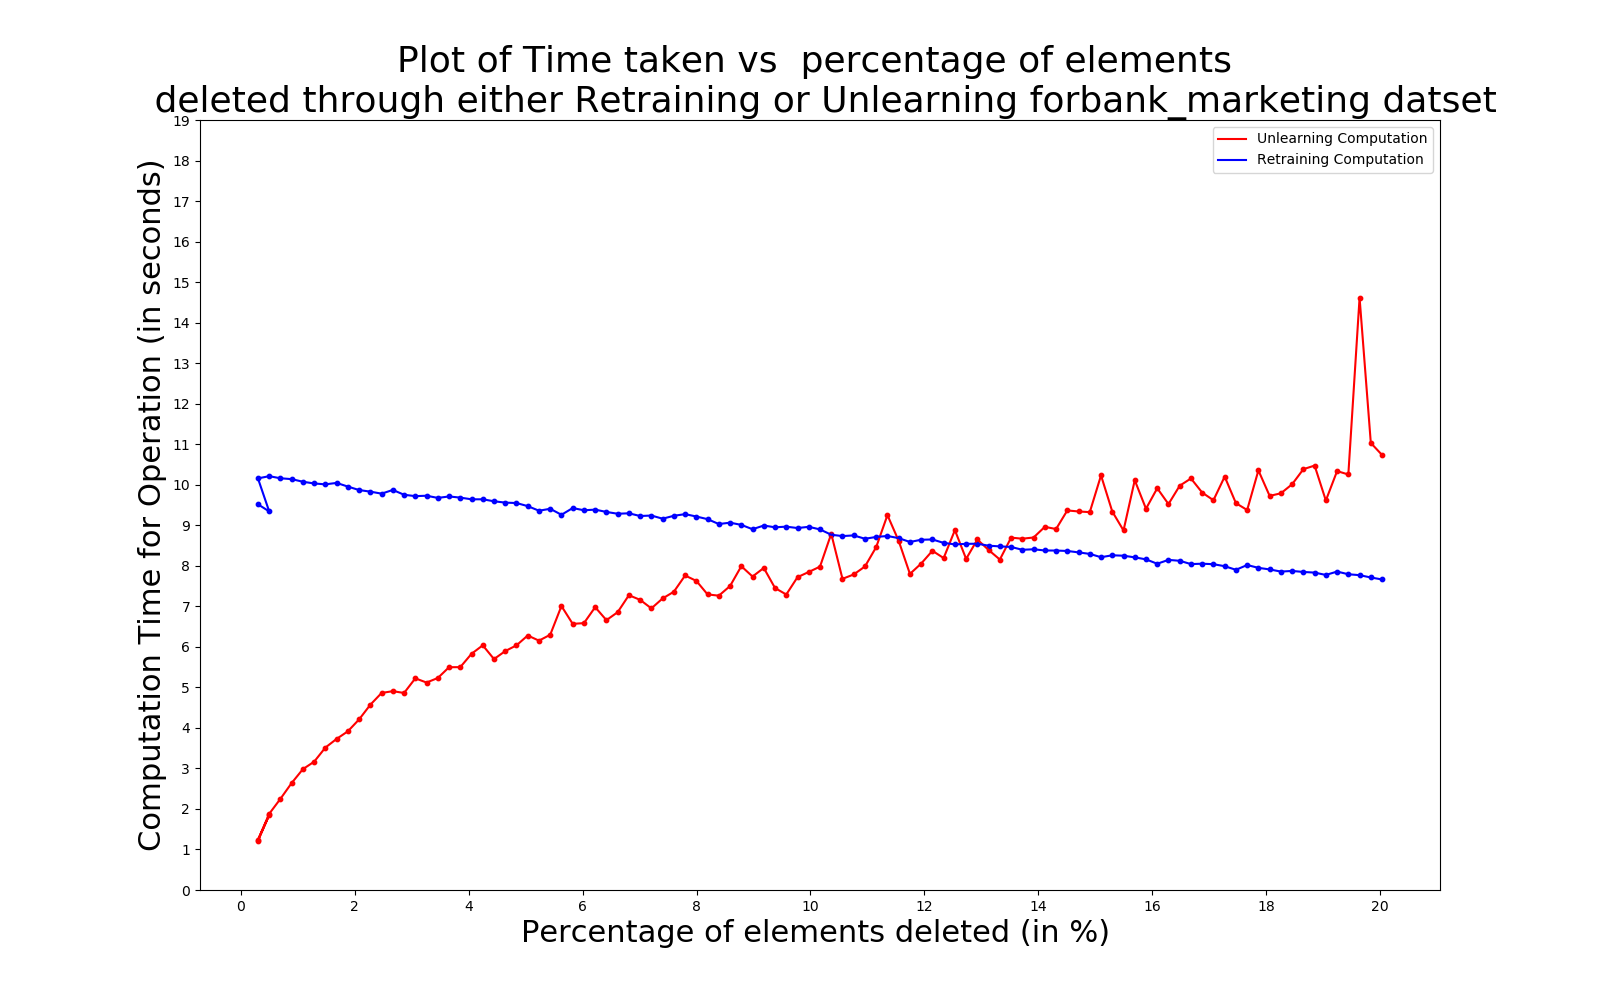
\includegraphics[width=6.5 in]{tables/PlotUnlearningVsRetrainingbank_marketing.png}
    \caption{Bank Marketing Dataset: Computation time as a function of percentage of elements deleted - for retraining vs unlearning}
    \label{fig:graph-bankmarketing}
\end{figure}

\begin{figure}[h]
    \centering
    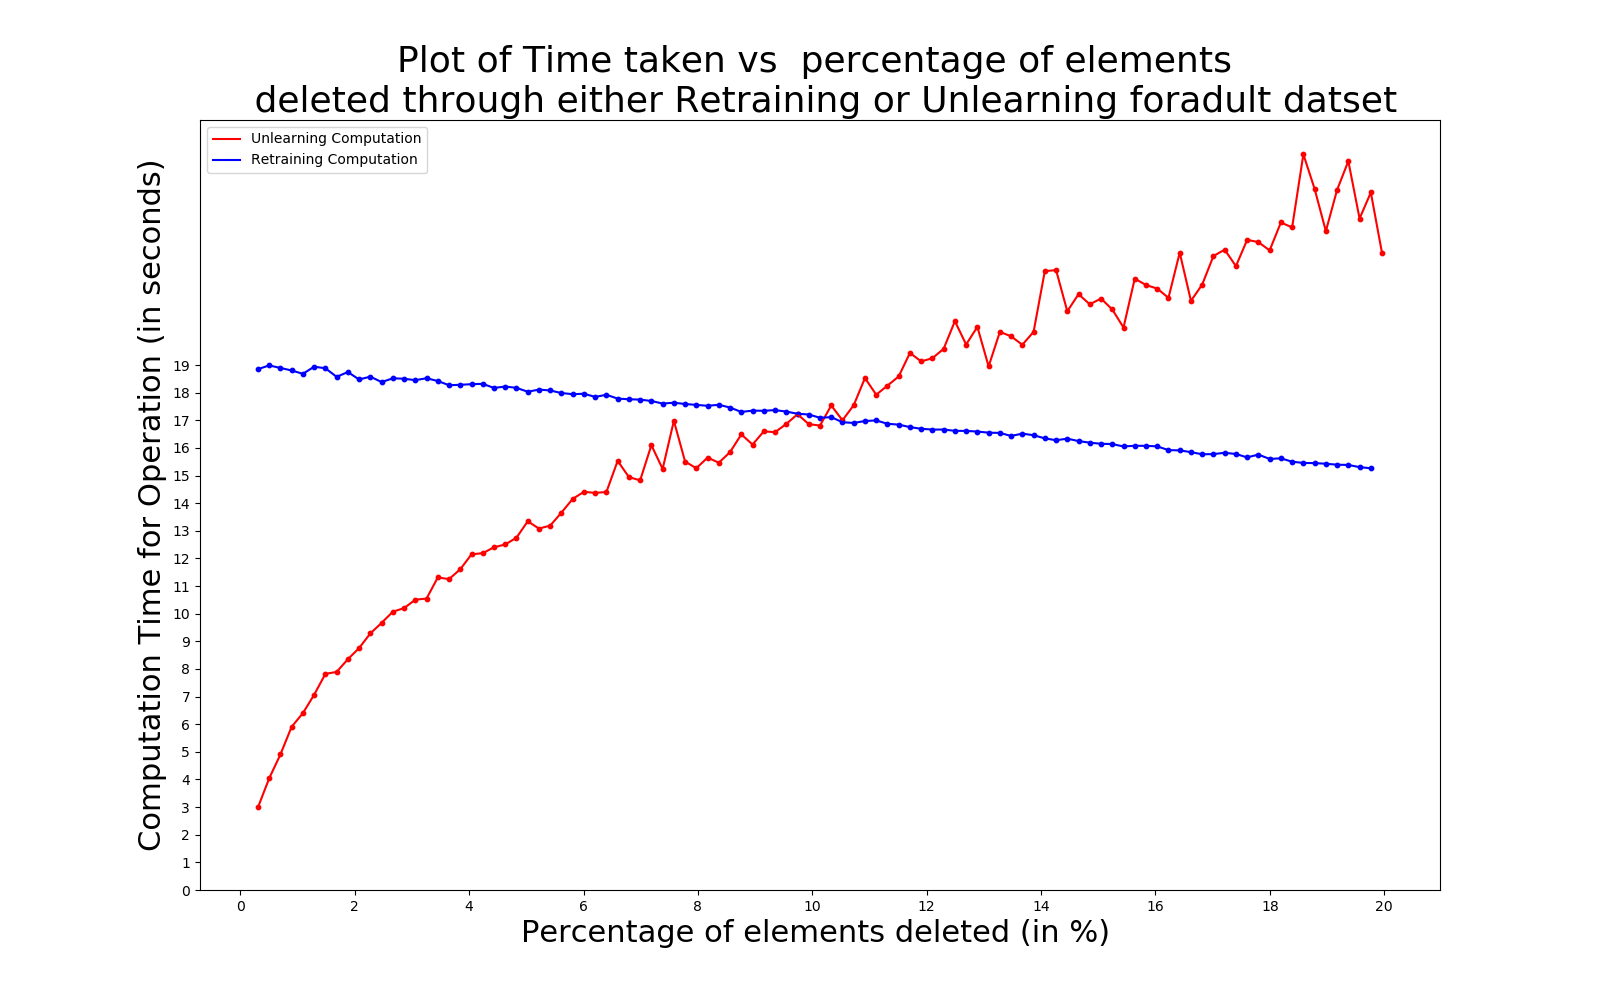
\includegraphics[width=6.5 in]{tables/PlotUnlearningVsRetrainingadult.png}
    \caption{Census Income Dataset: Computation time as a function of percentage of elements deleted - for retraining vs unlearning}
    \label{fig:graph-censusincome}
\end{figure}

\begin{figure}[h!]
    \centering
    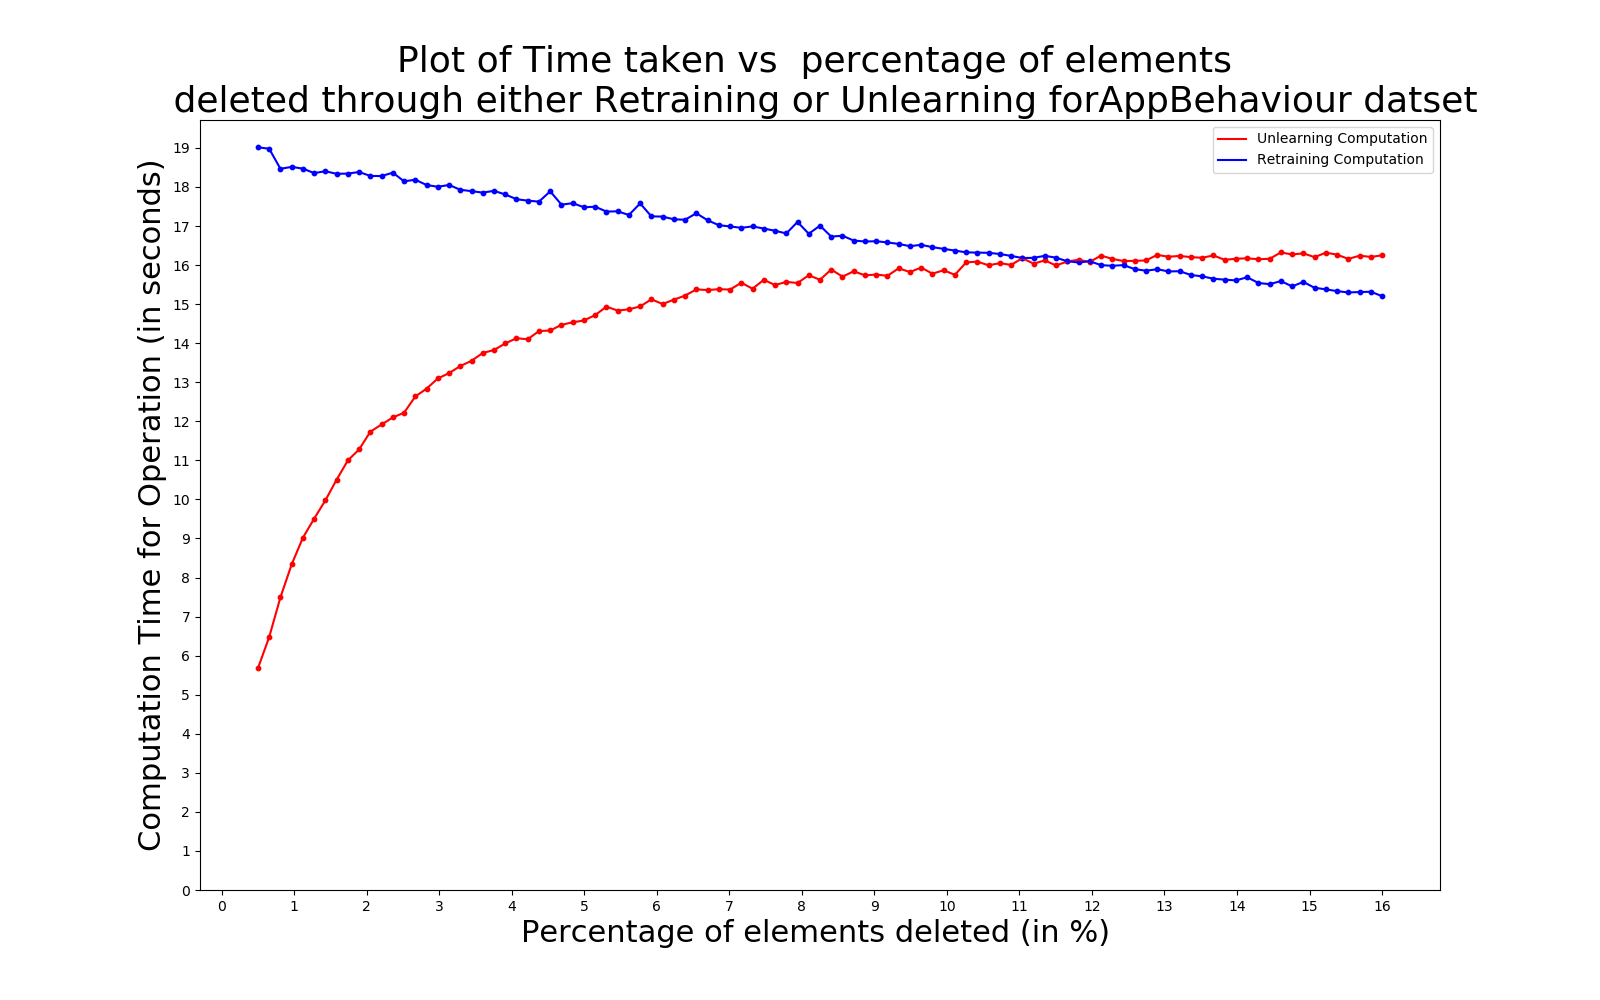
\includegraphics[width=6.5 in ]{tables/PlotUnlearningVsRetrainingAppBehaviour.png}
    \caption{App Behaviour Dataset: Computation time as a function of percentage of elements deleted - for retraining vs unlearning}
    \label{fig:graph-appbehaviour}
\end{figure}
\FloatBarrier

\section{Results}

\begin{itemize}
    \item Post unlearning we computed confusion matrix followed by precision, recall and accuracy scores. We compared the performance of unlearned model vs. completely retrained model for three datasets to produce the following results in the tables~\ref{fig:censusincome-results-1},~\ref{fig:bankmarketing-results-1} and~\ref{fig:appbehaviour-results-1} .
    \item We find that the generalization error does not vary significantly and the model is able to unlearn data in 3-4 orders of magnitude faster than retraining from scratch while sacrificing less than 1\% in terms of predictive performance for which results are reported in~\ref{fig:speeduptime}.
    \item We observed as we increase the number of indices to be removed the speedup is less significant as compared to retraining the left portion and its better to actually retrain rather than unlearn which roughly happens when unlearning around 11$\%$ of dataset as evident from the analysis of computation time with varying percentage of elements deleted for all three datasets referenced in~\ref{fig:graph-bankmarketing},~\ref{fig:graph-censusincome} and~\ref{fig:graph-appbehaviour}.
    \item Unlearning Time Speedup Analysis: We observed the improve in speedup for small data unlearning~\ref{fig:paramtuning}, but did not see the same results being reproduced as we increase the unlearning size shown.
    \item Space Computation Analysis: Our experimental findings match with the theoretical claims as we observed an overhead in space consumption by a factor of 3-10 when compared to the simple random forest by the scikit learn for which the results are~\ref{fig:memusagebankmarketing}, ~\ref{fig:memusagecensusincome} and~\ref{fig:memusageappbehviour}. 
    \item Membership Inference Attack Analysis: We formulated the attack accuracy results shown in~\ref{fig:MIA-attacks} and found that the attack accuracy results for Shokri and Loss Attack 2 are in the range (26\%-40\%) for all the three datasets. This complements the failure of the membership inference attacks to predict the deleted samples in or out of the training set. Considering the data deletions as exact in the DaRE models, membership inference attacks failed and hence we validated the claim by the researchers that \textit{data deletions in DaRE models are exact, membership inference attacks are guaranteed to be unsuccessful for instances deleted from the model}.
    
\end{itemize}    

\section{Conclusions \& Future work}

We have successfully implemented DaRE, tested its robustness and operating limits of unlearning by performing unlearning tests for varying deletion size (small, medium, large). We performed time and space analysis to understand DaRE and tuned hyper-parameters to avoid overfitting and improve the speedup in order to achieve threshold for optimal deletion greater than 11\%. After the hyper-parameter tuning, we noticed speedup in the unlearning for smaller data deletions but this difference does not translate to the large data deletions. We find that the claim holds true regarding membership inference attacks and membership inference attacks are unsuccessful on DaRE model under black box settings.

Future Work: We will try to bring down space overhead which will enhance the performance of DARE in 11+\% data unlearning cases. In addition to that, we want to implement and test differential-private random forest models, but the problem lies in the large privacy budget and generalization error due to which they often suffer from poor predictive performance.
\bibliography{refs}
\bibliographystyle{plain}


\end{document} % end tag of the document